% Options for packages loaded elsewhere
\PassOptionsToPackage{unicode}{hyperref}
\PassOptionsToPackage{hyphens}{url}
%
\documentclass[
]{article}
\usepackage{lmodern}
\usepackage{amssymb,amsmath}
\usepackage{ifxetex,ifluatex}
\ifnum 0\ifxetex 1\fi\ifluatex 1\fi=0 % if pdftex
  \usepackage[T1]{fontenc}
  \usepackage[utf8]{inputenc}
  \usepackage{textcomp} % provide euro and other symbols
\else % if luatex or xetex
  \usepackage{unicode-math}
  \defaultfontfeatures{Scale=MatchLowercase}
  \defaultfontfeatures[\rmfamily]{Ligatures=TeX,Scale=1}
\fi
% Use upquote if available, for straight quotes in verbatim environments
\IfFileExists{upquote.sty}{\usepackage{upquote}}{}
\IfFileExists{microtype.sty}{% use microtype if available
  \usepackage[]{microtype}
  \UseMicrotypeSet[protrusion]{basicmath} % disable protrusion for tt fonts
}{}
\makeatletter
\@ifundefined{KOMAClassName}{% if non-KOMA class
  \IfFileExists{parskip.sty}{%
    \usepackage{parskip}
  }{% else
    \setlength{\parindent}{0pt}
    \setlength{\parskip}{6pt plus 2pt minus 1pt}}
}{% if KOMA class
  \KOMAoptions{parskip=half}}
\makeatother
\usepackage{xcolor}
\IfFileExists{xurl.sty}{\usepackage{xurl}}{} % add URL line breaks if available
\IfFileExists{bookmark.sty}{\usepackage{bookmark}}{\usepackage{hyperref}}
\hypersetup{
  pdftitle={Who are you},
  pdfauthor={Bige Ozkan},
  hidelinks,
  pdfcreator={LaTeX via pandoc}}
\urlstyle{same} % disable monospaced font for URLs
\usepackage[margin=1in]{geometry}
\usepackage{graphicx,grffile}
\makeatletter
\def\maxwidth{\ifdim\Gin@nat@width>\linewidth\linewidth\else\Gin@nat@width\fi}
\def\maxheight{\ifdim\Gin@nat@height>\textheight\textheight\else\Gin@nat@height\fi}
\makeatother
% Scale images if necessary, so that they will not overflow the page
% margins by default, and it is still possible to overwrite the defaults
% using explicit options in \includegraphics[width, height, ...]{}
\setkeys{Gin}{width=\maxwidth,height=\maxheight,keepaspectratio}
% Set default figure placement to htbp
\makeatletter
\def\fps@figure{htbp}
\makeatother
\setlength{\emergencystretch}{3em} % prevent overfull lines
\providecommand{\tightlist}{%
  \setlength{\itemsep}{0pt}\setlength{\parskip}{0pt}}
\setcounter{secnumdepth}{-\maxdimen} % remove section numbering

\title{Who are you}
\author{Bige Ozkan}
\date{9/8/2021}

\begin{document}
\maketitle

\hypertarget{personal}{%
\section{Personal}\label{personal}}

I am an only-child who always wanted to have siblings. I still feel
grateful to my parents for letting me adopt a parakeet, a turtle, and
finally a dog. (this could have been a ``fun fact'')

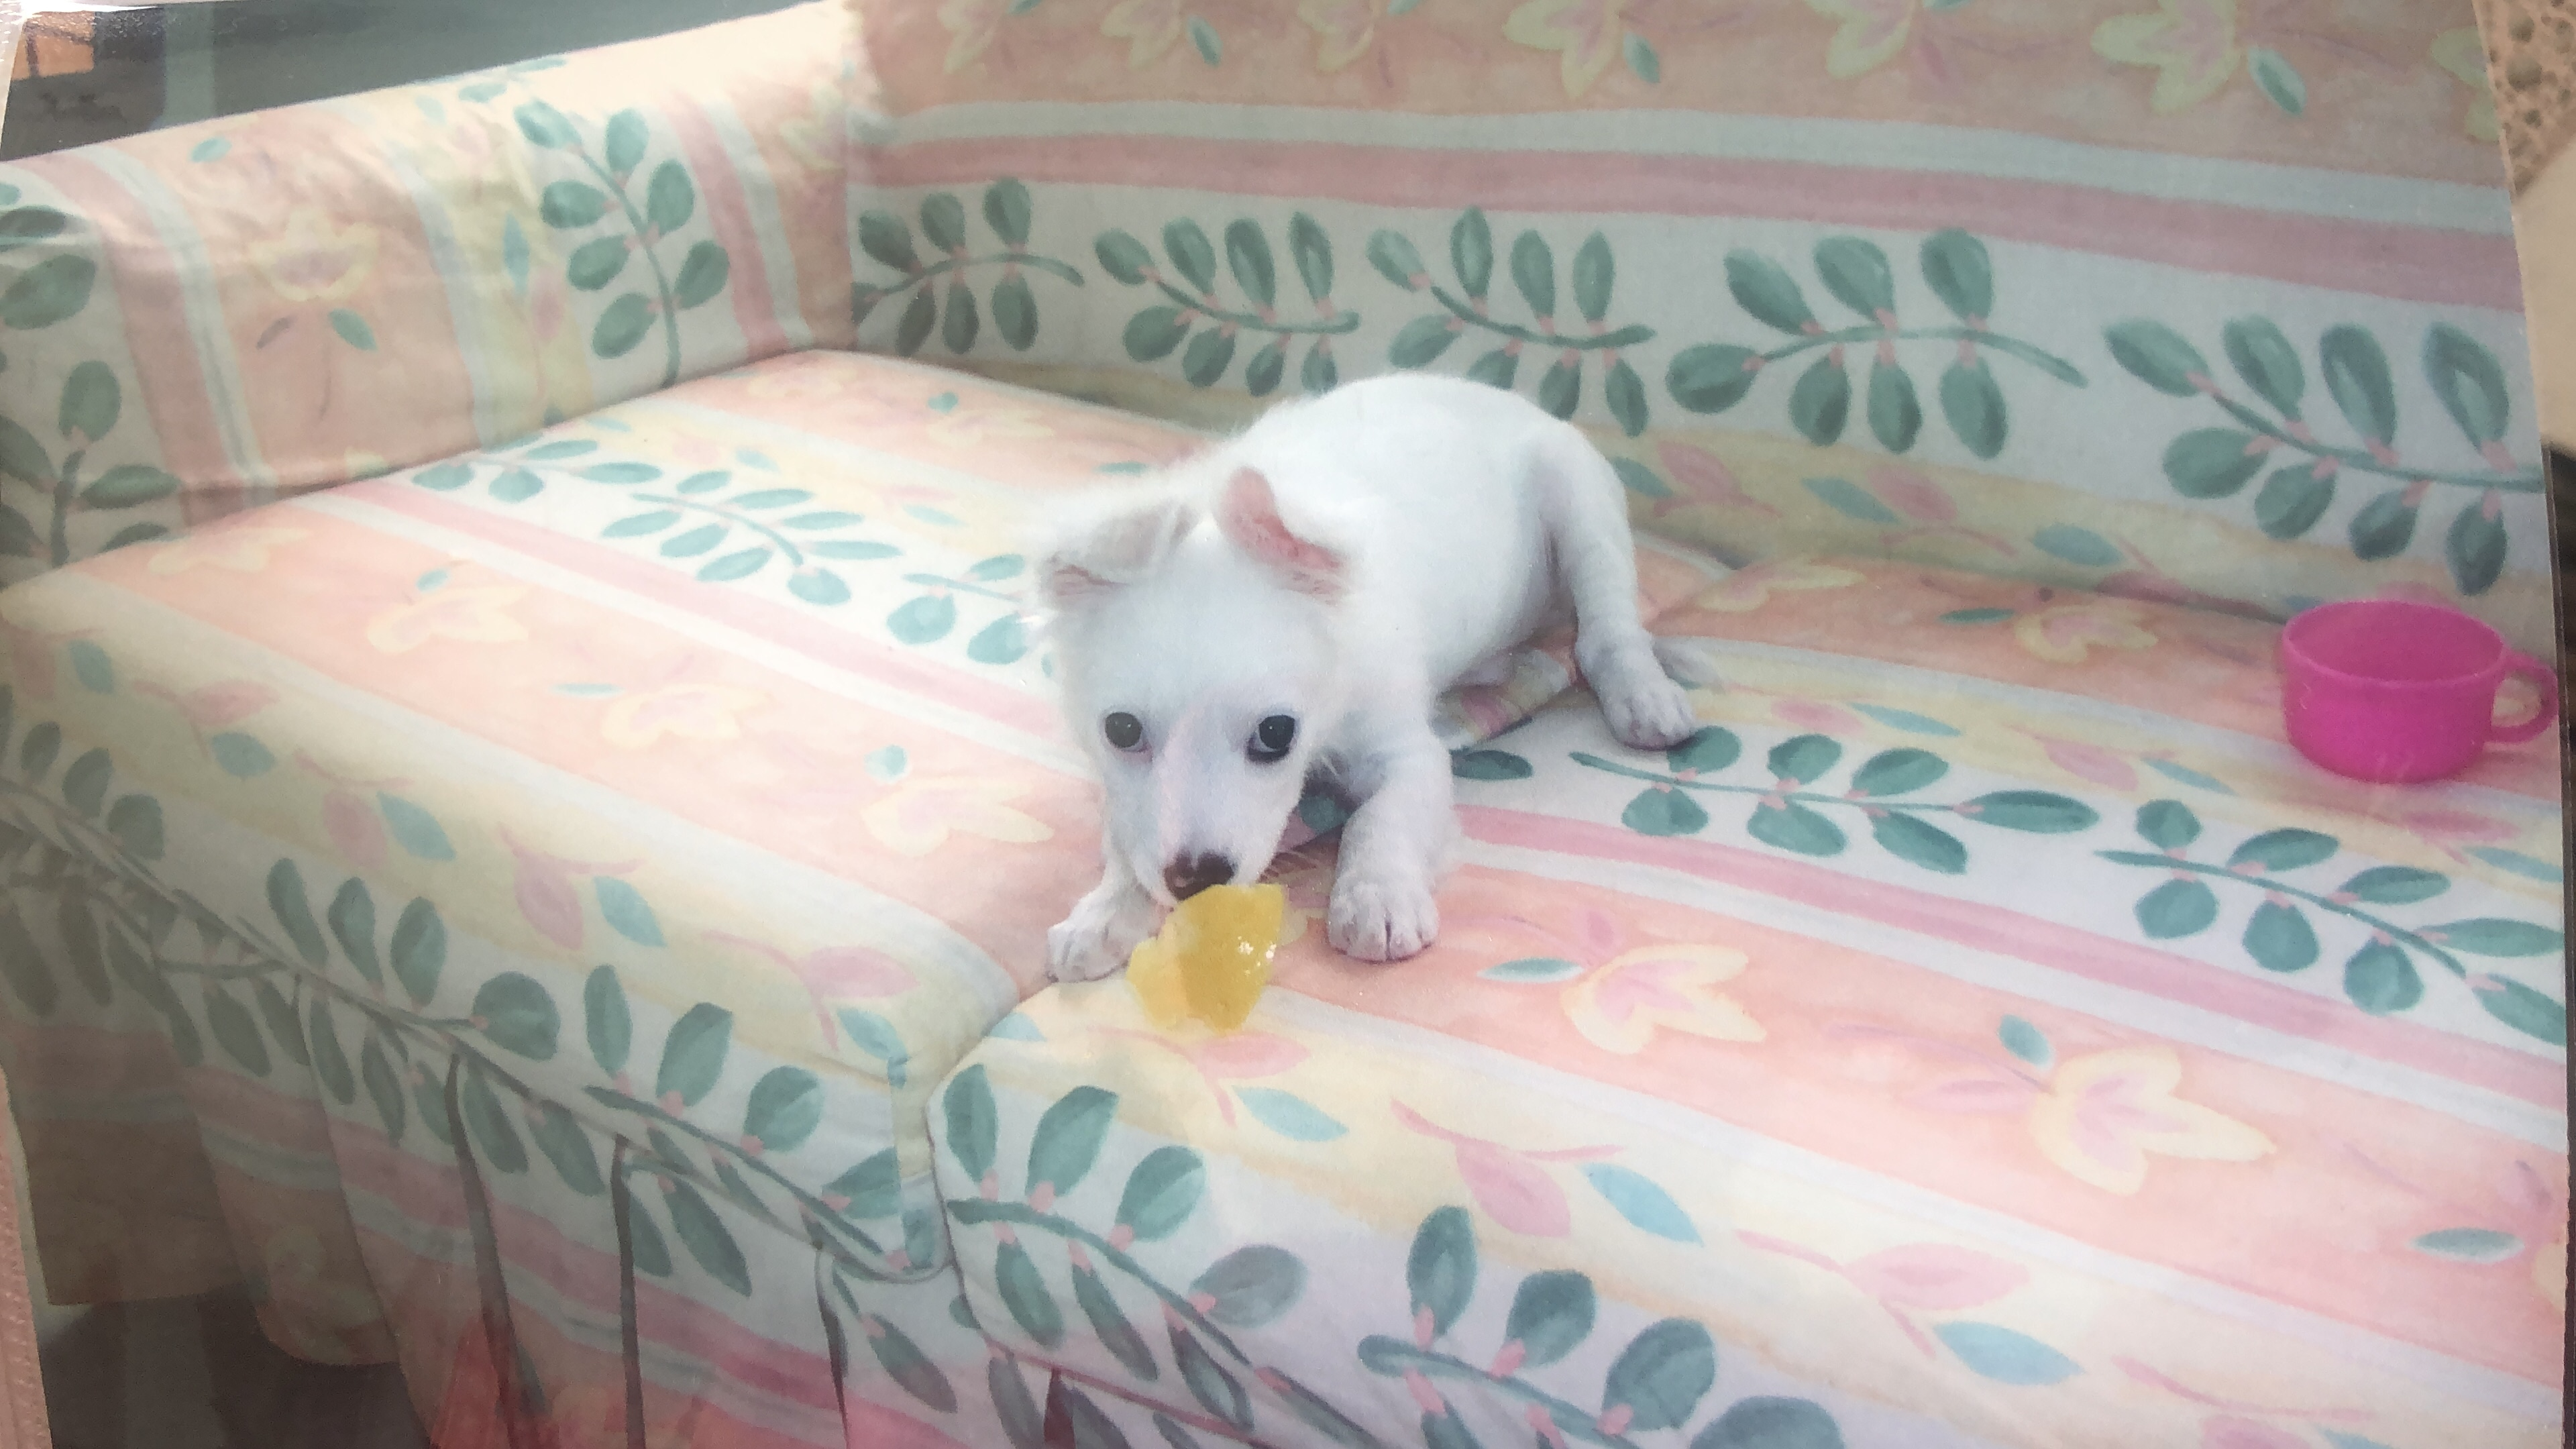
\includegraphics{/Users/bigeozkan/Documents/GitHub/biostat776-intro-bige-ozkan/biostat776-intro-bige-ozkan/pamuk_baby.jpg}
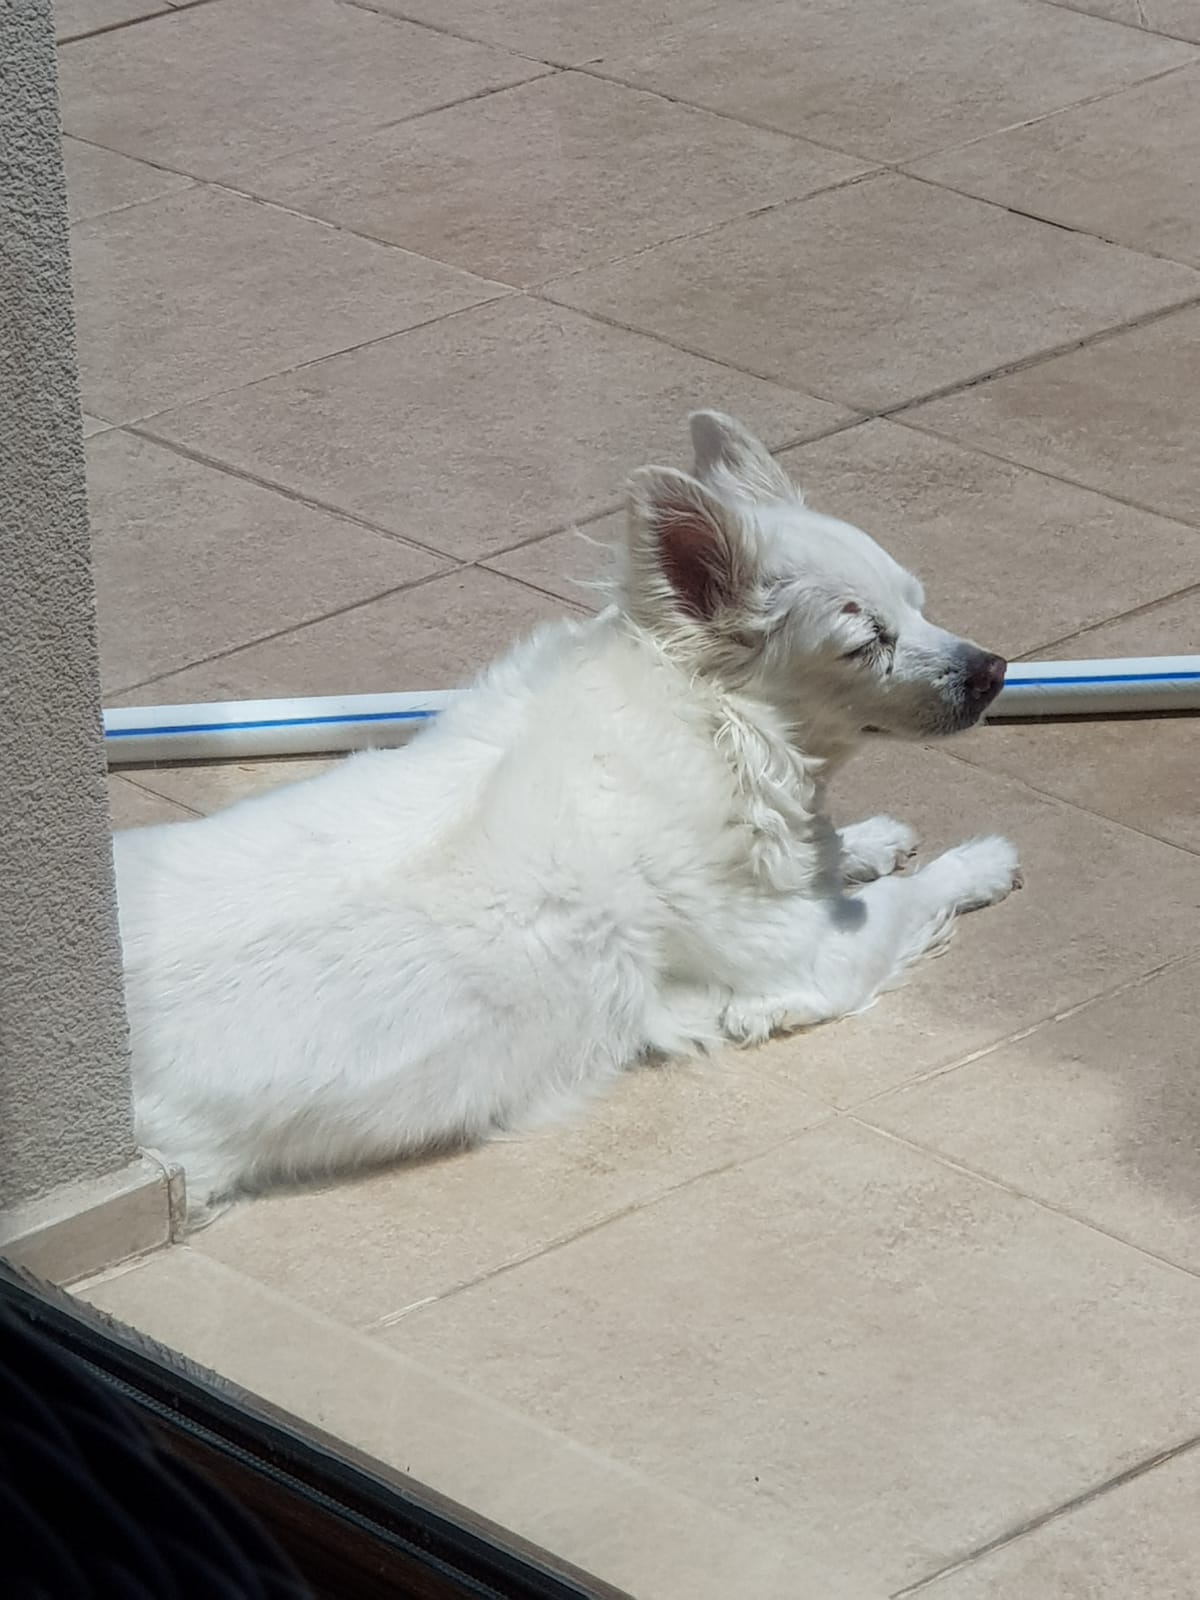
\includegraphics{/Users/bigeozkan/Documents/GitHub/biostat776-intro-bige-ozkan/biostat776-intro-bige-ozkan/pamuk_14.jpg}

\hypertarget{academic}{%
\section{Academic}\label{academic}}

\hypertarget{before}{%
\subsection{Before}\label{before}}

I went to medical school in Istanbul, Turkey, and graduated last year
(in 2020).

\hypertarget{now}{%
\subsection{Now}\label{now}}

I am a second year Master of Science student in Epidemiology, Clinical
and Cardiovascular Track. My main research interests are cardiovascular
diseases and risk factors (particularly that of heart failure) and use
of cardiac biomarkers for risk stratification.

\hypertarget{future}{%
\subsection{Future}\label{future}}

I am planning to pursue further clinical training in Internal Medicine
and Cardiology.

\hypertarget{statisticsdata-analysis-experience}{%
\section{Statistics/Data analysis
experience}\label{statisticsdata-analysis-experience}}

I have been using Stata for my research projects and conducted the
statistical analyses on my own, but I have always been very jealous of
the online support system of the R community.

\hypertarget{why-this-course-my-expectations}{%
\subsection{``Why this course'' \& My
expectations}\label{why-this-course-my-expectations}}

Because of my friends who mainly use R, I started to understand and
appreciate R's principle of open-source, reproducible research. Since I
want to become a physician-scientist, keeping up with the most useful
and powerful programs is essential. I want to be able to write and edit
my own code in R, in an organized fashion. I am also very interested in
data visualization and I am looking forward to learning more about
ggplots!

\end{document}
